\documentclass[11pt,a4paper]{article}

% ---------- Encoding and language ----------
\usepackage[T1]{fontenc}
\usepackage[utf8]{inputenc}
\usepackage[english]{babel}

% ---------- Mathematics ----------
\usepackage{amsmath,amssymb,amsthm,mathtools}
\usepackage{bm}

% ---------- Layout ----------
\usepackage[margin=2.5cm]{geometry}
\usepackage[protrusion=true,expansion=false]{microtype}
\usepackage{booktabs}
\usepackage{graphicx}
\usepackage{enumitem}
\usepackage{xcolor}
\usepackage{listings}
\usepackage{tikz}
\usepackage[colorlinks=true,linkcolor=blue!50!black,citecolor=green!50!black,urlcolor=blue!60!black]{hyperref}

% ---------- Theorem environments ----------
\theoremstyle{plain}
\newtheorem{theorem}{Theorem}[section]
\newtheorem{proposition}[theorem]{Proposition}
\newtheorem{lemma}[theorem]{Lemma}
\newtheorem{hypothesis}{Hypothesis}
\theoremstyle{definition}
\newtheorem{definition}[theorem]{Definition}
\newtheorem{conjecture}[theorem]{Conjecture}
\theoremstyle{remark}
\newtheorem{remark}[theorem]{Remark}

% ---------- Operators and shorthands ----------
\DeclareMathOperator{\vol}{vol}
\DeclareMathOperator*{\argmin}{arg\,min}
\newcommand{\core}{\mathrm{core}}
\newcommand{\giant}{\mathrm{giant}}
\newcommand{\periph}{\mathrm{periph}}
\newcommand{\modu}{\mathrm{mod}}
\newcommand{\Ph}{\varphi}
\newcommand{\dmin}{d_{\min}}
\newcommand{\dmax}{d_{\max}}
\newcommand{\dbar}{\bar d}
\newcommand{\lamtwo}{\lambda_2}
\newcommand{\lamthree}{\lambda_3}
\newcommand{\Gcore}{G_{\core}}
\newcommand{\Ggiant}{G_{\giant}}
\newcommand{\Gtwo}{G_{2\core}}

% ---------- Listings ----------
\lstset{
  basicstyle=\ttfamily\small,
  keywordstyle=\color{blue!60!black},
  commentstyle=\color{green!45!black},
  stringstyle=\color{red!60!black},
  showstringspaces=false,
  breaklines=true,
  frame=single,
  language=Python
}

% =====================================================================
\title{\bfseries The Spectral Gap of the Normalized Laplacian\\
in Sparse Heavy-Tailed Random Graphs:\\
Asymptotics, Bottleneck Structure, and Modularity\\
in Biological Networks}

\author{Leonid L.~Kuzmin\\[2pt]
\small M.Sc.\\
\small\href{mailto:kuzminll@vk.com}{kuzminll@vk.com}}
\date{\today}

\begin{document}
\maketitle

\begin{abstract}
\noindent
We study the second eigenvalue $\lamtwo$ of the normalized Laplacian
$L=I-D^{-1/2}AD^{-1/2}$ in sparse random graphs with a heavy-tailed degree
distribution $P(D=k)\sim Ck^{-\gamma}$ in the regime $\dbar_{\min}=O(1)$,
which is not covered by the classical Chung--Lu--Vu theory. We argue that the
exponent $\gamma$ alone is insufficient: the order of $\lamtwo$ is determined
by the competition of three scales --- low-degree periphery, modular cuts, and
hubs/the core. We introduce a diagnostic system consisting of the conductance
ratio $\Delta=\Ph_{\modu}/\Ph_{\periph}$, the volume fraction $\rho_*$ of the
minimal cut, the localization of the second eigenvector measured by the inverse
participation ratio $\mathrm{IPR}(v_2)$, and the full sweep-cut conductance
profile $\Ph(\rho)$. These quantities distinguish a peripheral bottleneck from
macroscopic modularity and from a core-dominated regime. We propose a phase
diagram in the coordinates $(\log\Delta,\rho_*)$ and a computational protocol
for constructing it, and we discuss a careful biological interpretation: a
small $\lamtwo$ by itself does not identify functional modularity.
\end{abstract}

\noindent\textbf{Keywords:} normalized Laplacian; spectral gap; heavy-tailed
degree distribution; configuration model; conductance; Cheeger inequality;
eigenvector localization; modularity; biological networks.

\tableofcontents

% =====================================================================
\section{Introduction and Motivation}
\label{sec:motivation}

\textbf{Starting point.} The goal is to obtain the exact asymptotics of the
second eigenvalue $\lamtwo$ of the normalized Laplacian for sparse random
graphs with a heavy-tailed degree distribution $P(D=k)\sim Ck^{-\gamma}$ in the
regime $\dbar_{\min}=O(1)$, which lies outside the scope of the
Chung--Lu--Vu theorem.

\textbf{Problem with the naive formulation.} The statement is too broad and,
for some parameter values, trivially false. In the sparse regime $\lamtwo$ may
be zero because the graph is disconnected, and after removing small components
it may have a completely different order of magnitude. This is not a technical
detail but a central part of the problem.

\textbf{Correction.} Instead of a single formula
$\lamtwo\sim f(\gamma,\dbar,n)$ one must build a \emph{phase diagram for the
order of $\lamtwo$} as a function of
\begin{equation}
\gamma,\qquad \dmin,\qquad \dmax,\qquad \dbar,\qquad n,
\end{equation}
and, most importantly, of the \emph{structure of the low-degree tail}.

% =====================================================================
\section{Known Results}
\label{sec:known}

\begin{itemize}[leftmargin=*]
\item \textbf{Chung--Lu--Vu \cite{ChungLuVu2003}.} For random graphs with
prescribed expected degrees, when $\dbar_{\min}\gg\ln^2 n$ the spectrum of the
normalized Laplacian concentrates around the predicted behaviour; the results
include power-law graphs. The gap estimate reads
\begin{equation}
\lambda(G)\;\ge\;1-4\,\dbar^{-1/2}-\dbar_{\min}^{-1}\ln^2 n .
\label{eq:CLV}
\end{equation}
For $\dbar_{\min}\le\ln^2 n$ the bound \eqref{eq:CLV} becomes vacuous.

\item \textbf{Coja-Oghlan--Lanka \cite{CojaLanka2009}.} In the sparse regime
$\dbar_{\min}=O(1)$ there exists a large core whose spectral gap of the
normalized Laplacian stays separated from zero:
\begin{equation}
\lamtwo(L_{\core})\;\ge\;1-c_0\,\dbar_{\min}^{-1/2}
\label{eq:COL}
\end{equation}
with high probability. The statement concerns the \emph{core}, not the whole
graph.

\item \textbf{For $G(n,p)$ with bounded average degree $d$.} The spectral gap
of the whole graph satisfies $\lamtwo=o(1)$, whereas the giant component or the
core may have a gap of order one.
\end{itemize}

\begin{remark}[key consequence]
\begin{equation}
\boxed{\;\lamtwo(G)\;\not\sim\;\lamtwo(\core(G)).\;}
\end{equation}
\end{remark}

% =====================================================================
\section{Why the Exponent $\gamma$ Alone Is Insufficient}
\label{sec:gamma}

Let $P(D=k)\sim Ck^{-\gamma}$. This determines the tail for large $k$, but
$\lamtwo$ is highly sensitive to \emph{small degrees}.

\textbf{Counterexample.} Two degree sequences with the same $\gamma=2.5$:
\begin{itemize}[leftmargin=*]
\item model A: $P(D=1)>0$;
\item model B: $P(D=1)=0,\;P(D\ge 2)=1$.
\end{itemize}
They have the same asymptotic tail but completely different behaviour of
$\lamtwo$. Model A produces leaves and finite components; model B may be
substantially more connected.
\begin{equation}
\boxed{\;\gamma\ \text{does not determine}\ \lamtwo.\;}
\end{equation}

\textbf{A hard counterexample.} Consider a configuration model with
$P(D=1)=p_1>0$. At bounded average degree such graphs naturally contain small
components and dangling structures. If the graph is disconnected then
$\lamtwo(L)=0$. Consequently, no nontrivial formula of the form
$\lamtwo\sim f(\gamma)>0$ can hold for the whole graph.

% =====================================================================
\section{Three Spectral Gaps}
\label{sec:three}

\begin{table}[h]
\centering
\begin{tabular}{llp{7.2cm}}
\toprule
Object & Notation & What it captures \\
\midrule
Whole graph & $\lamtwo(G)$ & Global connectivity; $\lamtwo=0$ if disconnected \\
Giant component & $\lamtwo(\Ggiant)$ & The meaningful quantity for sparse heavy-tailed networks \\
2-core & $\lamtwo(\Gtwo)$ & A nonzero asymptotic lower bound even for $\dbar_{\min}=O(1)$ \\
\bottomrule
\end{tabular}
\caption{The three levels of the spectral gap.}
\end{table}

\begin{hypothesis}[ordering of the gaps]
\begin{equation}
\boxed{\;\lamtwo(G)\;\ll\;\lamtwo(\Ggiant)\;\lesssim\;\lamtwo(\Gtwo).\;}
\end{equation}
\end{hypothesis}

% =====================================================================
\section{Three Mechanisms Producing a Small $\lamtwo$}
\label{sec:mechanisms}

\begin{enumerate}[leftmargin=*]
\item \textbf{Small components:} $\lamtwo(G)=0$.
\item \textbf{Dangling trees:} long ``whiskers'' create a small conductance;
by Cheeger's inequality $\lamtwo\le 2\Ph$, so a sufficiently long thin pendant
structure can drive $\lamtwo\to 0$.
\item \textbf{Genuine modularity:} two large dense communities joined by a
small cut give $\Ph\ll 1$ and hence $\lamtwo\ll 1$.
\end{enumerate}

\textbf{Key distinction.}
\begin{equation}
\text{small }\lamtwo\ \Longrightarrow\ \text{a weak global cut exists},
\end{equation}
but
\begin{equation}
\text{small }\lamtwo\ \not\Longrightarrow\ \text{biological modularity}.
\end{equation}
One must separate a \emph{community bottleneck} from a \emph{peripheral
bottleneck}.

% =====================================================================
\section{Two Types of Bottleneck}
\label{sec:bottleneck}

Let
\begin{equation}
\vol(S)=\sum_{v\in S}d_v,\qquad
\Ph(S)=\frac{|\partial S|}{\vol(S)} .
\end{equation}

\begin{definition}[peripheral bottleneck]
\begin{equation}
\Ph_{\periph}(G)=
\min_{\substack{S\subset V\\ 0<\vol(S)\le\varepsilon\,\vol(V)}}\Ph(S),
\end{equation}
where $\varepsilon\ll 1$, for example $\varepsilon=0.05$.
\end{definition}

\begin{definition}[modular bottleneck]
\begin{equation}
\Ph_{\modu}(G)=
\min_{\substack{S\subset V\\ \varepsilon\,\vol(V)\le\vol(S)\le\frac12\vol(V)}}\Ph(S).
\end{equation}
\end{definition}

Hence
\begin{equation}
\Ph(G)=\min\{\Ph_{\periph},\Ph_{\modu}\}.
\end{equation}
By Cheeger's inequality \cite{Cheeger1970,KannanVempalaVetta2004},
\begin{equation}
\frac{\Ph(G)^2}{2}\;\le\;\lamtwo\;\le\;2\,\Ph(G).
\label{eq:cheeger}
\end{equation}
Thus we obtain not a ``decomposition of $\lamtwo$'' but a \emph{classification
of the mechanism that creates the global bottleneck}.

% =====================================================================
\section{Diagnostic Parameters}
\label{sec:diagnostics}

\begin{definition}[competition parameter]
\begin{equation}
\boxed{\;\Delta(G)=\frac{\Ph_{\modu}(G)}{\Ph_{\periph}(G)}\;}
\end{equation}
\end{definition}
with the interpretation:
\begin{itemize}[leftmargin=*]
\item $\Delta\gg 1$ --- the peripheral bottleneck is cheaper;
\item $\Delta\ll 1$ --- the modular bottleneck is cheaper;
\item $\Delta\approx 1$ --- a transitional regime.
\end{itemize}
For numerical stability we work with
\begin{equation}
\log\Delta=\log\Ph_{\modu}-\log\Ph_{\periph}.
\end{equation}

\begin{definition}[scale of the minimal cut]
\begin{equation}
\rho(S)=\frac{\vol(S)}{\vol(V)},\qquad
\rho_*=\rho(S_*),\qquad
S_*=\argmin_{S}\Ph(S).
\end{equation}
\end{definition}
Interpretation:
\begin{itemize}[leftmargin=*]
\item $\rho_*=O(n^{-1})$ --- a small local structure;
\item $\rho_*=O(1)$ --- a macroscopic separation of the graph.
\end{itemize}

\textbf{Spectral versus combinatorial cut.}
\begin{equation}
\rho_2=\frac{\vol(\{v:f_2(v)>0\})}{\vol(V)} .
\end{equation}
If $\rho_2\approx\rho_*$ the spectral cut coincides with the combinatorial one;
otherwise $\lamtwo$ is controlled not by the minimal cut but by an ``averaged''
behaviour.

\textbf{Multiple bottlenecks.} The difference $\lamthree-\lamtwo$: a small
difference indicates several competing cuts of similar conductance. This is a
useful symptom but not a criterion; it must be complemented by the localization
of the eigenvectors.

\begin{definition}[localization of the second eigenvector]
\begin{equation}
\mathrm{IPR}_2(v)=\frac{\sum_i v_i^4}{\left(\sum_i v_i^2\right)^2},
\qquad
\mathrm{IPR}_2^{\pi}(v)=\sum_i w_i^2,\quad
w_i\propto\pi_i\,v_i^2,
\end{equation}
where $\pi_i=d_i/\vol(V)$ is the stationary measure of the random walk.
\end{definition}
Interpretation:
\begin{itemize}[leftmargin=*]
\item a delocalized mode (modularity, macroscopic cut): $\mathrm{IPR}_2\sim 1/n$;
\item a localized mode (periphery): $\mathrm{IPR}_2\sim 1/k$ on a support of
size $k$; an estimate of the support is $\mathrm{PR}_2=1/\mathrm{IPR}_2$.
\end{itemize}
\begin{remark}
The IPR is informative only when $\lamtwo$ is \emph{non-degenerate}. If
$\lamtwo$ has high multiplicity (for instance $n-1$ for $K_n$), the eigenvector
is not unique and the IPR is not well defined.
\end{remark}

\textbf{Conductance profile.} Instead of a fixed threshold $\varepsilon$ one may
use the full sweep-cut profile $\Ph(\rho)$ along $f_2$ in both directions and
identify the regimes \emph{post hoc}.

\textbf{Diagnostic space:} $(\log\Delta,\rho_*,\mathrm{IPR}_2)$.

% =====================================================================
\section{Phase Diagram (Hypothetical)}
\label{sec:phase}

\begin{figure}[h]
\centering
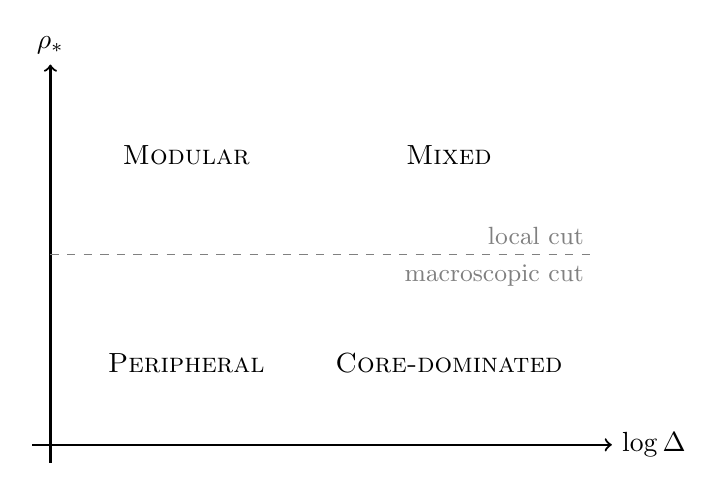
\begin{tikzpicture}[scale=1.15]
\draw[->,thick] (-0.2,0) -- (6.2,0) node[right] {$\log\Delta$};
\draw[->,thick] (0,-0.2) -- (0,4.2) node[above] {$\rho_*$};
\draw[dashed,gray] (0,2.1) -- (6.0,2.1);
\node[align=center] at (1.5,3.2) {\textsc{Modular}};
\node[align=center] at (4.4,3.2) {\textsc{Mixed}};
\node[align=center] at (1.5,0.9) {\textsc{Peripheral}};
\node[align=center] at (4.4,0.9) {\textsc{Core-dominated}};
\node[gray,anchor=north east] at (6.0,2.1) {\small macroscopic cut};
\node[gray,anchor=south east] at (6.0,2.1) {\small local cut};
\end{tikzpicture}
\caption{Hypothetical phase diagram in the coordinates
$(\log\Delta,\rho_*)$.}
\label{fig:phase}
\end{figure}

% =====================================================================
\section{Hypotheses}
\label{sec:hypotheses}

\begin{hypothesis}[H1]
For a sparse heavy-tailed configuration model with $P(D=k)\sim k^{-\gamma}$,
the asymptotics of $\lamtwo(G)$ is determined not by $\gamma$ alone but by the
competition of three scales:
\begin{equation}
\text{low-degree structures}\ \leftrightarrow\
\text{community cuts}\ \leftrightarrow\
\text{hub/core structure}.
\end{equation}
\end{hypothesis}

\begin{hypothesis}[H2]
For the whole graph, in the presence of a positive fraction of low-degree
vertices, $\lamtwo(G)\to 0$ may be a trivial consequence of the periphery or of
disconnection.
\end{hypothesis}

\begin{hypothesis}[H3]
After passing to the giant component or the 2-core, $\lamtwo(\Gtwo)$ may remain
separated from zero in a regime where the classical Chung--Lu--Vu theory
\cite{ChungLuVu2003} is not applicable.
\end{hypothesis}

\begin{hypothesis}[H4]
If a planted modular structure is added, a different scale appears:
\begin{equation}
\lamtwo\asymp\Ph_{\mathrm{module}}
\end{equation}
up to squared or linear factors dictated by Cheeger's inequality
\eqref{eq:cheeger}.
\end{hypothesis}

% =====================================================================
\section{Target Results}
\label{sec:result}

\textbf{Target theorem.}
\begin{equation}
\lamtwo(G_n)=\Theta\bigl(f(n,\gamma)\bigr)
\end{equation}
in a suitable regime. Separately,
\begin{equation}
\lamtwo(G_n^{2\core})=\Theta\bigl(g(\gamma,\dbar)\bigr)
\end{equation}
under different assumptions. If an exact asymptotic law cannot be obtained,
then
\begin{equation}
c\,f(n,\gamma)\;\le\;\lamtwo\;\le\;C\,f(n,\gamma)
\end{equation}
is already a complete result.

% =====================================================================
\section{Mathematical Setup}
\label{sec:setup}

The configuration model
\cite{BenderCanfield1978,MolloyReed1995,MolloyReed1998} with a deterministic
degree sequence $d_1,\dots,d_n$:
\begin{equation}
\sum_i d_i\equiv 0 \pmod 2,\qquad
N_k(n)=\#\{i:d_i=k\}\sim c\,n\,k^{-\gamma}.
\end{equation}
We vary
\begin{equation}
\dmin=1,2,3,\dots,\qquad
\dmax\sim n^{1/(\gamma-1)}
\end{equation}
or use a controlled cutoff.

\textbf{Methods:} message-passing approaches for arbitrary degree
distributions; spectral methods for configuration models
\cite{DorogovtsevGoltsevMendesSamukhin2003,Soderberg2002,BordenaveLelargeMassoulie2018}.

% =====================================================================
\section{Numerical Experiments}
\label{sec:experiments}

For each $(n,\gamma,\dmin)$ we generate $\approx 100$ realizations with
$n=10^3,10^4,10^5,\dots$ (and additional small sizes $n=100,\dots$ to probe the
transitional regime). For each realization we compute
\begin{align}
&\lamtwo(G),\quad \lamtwo(\Ggiant),\quad \lamtwo(\Gtwo),\\
&\Ph(G),\quad \Ph(\Ggiant),\quad \Ph(\Gtwo),\\
&\dmax,\quad \dbar,\quad N_1,\quad N_2 .
\end{align}
We also record $\Delta$, $\rho_*$, $\rho_2$, $\lamthree-\lamtwo$,
$\mathrm{IPR}_2(v_2)$ and the conductance profile $\Ph(\rho)$.

\textbf{Scaling.} We plot $\log\lamtwo$ against $\log n$. If
$\lamtwo\sim n^{-\alpha}$ then
\begin{equation}
\log\lamtwo=-\alpha\log n+C,
\end{equation}
and $\alpha$ is estimated statistically. We separately estimate the exponent in
$\lamtwo\sim(\Ph_*)^\alpha$; by Cheeger's inequality \eqref{eq:cheeger} one
expects $\alpha\in[1,2]$ when $\Ph_*$ is the controlling conductance.

\begin{table}[h]
\centering
\begin{tabular}{lp{8.5cm}}
\toprule
Ensemble & What we test \\
\midrule
Power-law $\dmin=1$ & periphery \\
Power-law $\dmin=2$ & chains / 2-core \\
Power-law $\dmin=3$ & expander-like core \\
Power-law $+$ planted communities & genuine modularity \\
\bottomrule
\end{tabular}
\caption{The four experimental ensembles.}
\end{table}

\begin{remark}
For $\dmin\ge 2$ there are no leaves, hence the 2-core coincides with the whole
graph: $G_{2\core}=G$ (up to disconnected small components). The core analysis
is therefore non-trivial only when low-degree vertices are present, i.e.\
essentially for $\dmin=1$.
\end{remark}

% =====================================================================
\section{Computing $\Ph_{\periph}$ and $\Ph_{\modu}$}
\label{sec:algorithm}

\subsection*{Approach 1: spectral approximation via sweep cut}

\begin{enumerate}[leftmargin=*]
\item Compute the second eigenvector $f_2$ of the normalized Laplacian
$L=I-D^{-1/2}AD^{-1/2}$.
\item Sort the vertices by $f_2(v)$: $v_1,\dots,v_n$.
\item Sweep cut: for each $k=1,\dots,n-1$ consider
$S_k=\{v_1,\dots,v_k\}$ and evaluate $\Ph(S_k)$.
\item Locate the minima:
\begin{align}
\Ph_{\periph}^{\mathrm{spec}}
&=\min\{\Ph(S_k):\vol(S_k)\le\varepsilon\vol(V)\},\\
\Ph_{\modu}^{\mathrm{spec}}
&=\min\{\Ph(S_k):\varepsilon\vol(V)\le\vol(S_k)\le\tfrac12\vol(V)\}.
\end{align}
\item Record the corresponding $\rho_*$.
\end{enumerate}
\textbf{Complexity:} $O(m\cdot\mathrm{iter}+n\log n)$.

\subsection*{Approach 2: local Cheeger with seed sets}

\begin{enumerate}[leftmargin=*]
\item Choose seed sets (low-degree vertices for the periphery; hubs or random
vertices for modularity).
\item Apply local clustering to each seed (Andersen--Chung--Lang,
PageRank-based) \cite{AndersenChungLang2006}.
\item Collect all found sets $S$ and evaluate $\Ph(S)$.
\item Filter by volume.
\end{enumerate}
\textbf{Complexity:} $O(nm\log n/\Ph^2)$.

\textbf{Recommendation.} Start with the spectral sweep cut. If
$\rho_2\ne\rho_*$, add local clustering for verification.

% =====================================================================
\section{Sweep-Cut Pseudocode}
\label{sec:pseudocode}

\begin{lstlisting}
import numpy as np
from scipy.sparse.linalg import eigsh

def spectral_diagnostics(L, degrees, adj, eps=0.05):
    n = len(degrees)
    vol_V = degrees.sum()

    vals, vecs = eigsh(L, k=2, which='SM')
    lambda2 = vals[1]
    f2 = vecs[:, 1]

    order = np.argsort(f2)

    vol_S = 0
    cut_size = 0
    in_S = np.zeros(n, dtype=bool)

    phi_periph = np.inf
    phi_mod = np.inf
    rho_periph = None
    rho_mod = None

    for k in range(n - 1):
        v = order[k]
        in_S[v] = True
        vol_S += degrees[v]

        for u in adj[v]:
            if in_S[u]:
                cut_size -= 1
            else:
                cut_size += 1

        if vol_S == 0:
            continue
        phi = cut_size / vol_S

        if vol_S <= eps * vol_V:
            if phi < phi_periph:
                phi_periph = phi
                rho_periph = vol_S / vol_V
        elif vol_S <= 0.5 * vol_V:
            if phi < phi_mod:
                phi_mod = phi
                rho_mod = vol_S / vol_V

    log_Delta = np.log(phi_mod) - np.log(phi_periph) if phi_periph > 0 else np.inf

    return {'lambda2': lambda2, 'phi_periph': phi_periph,
            'phi_mod': phi_mod, 'rho_periph': rho_periph,
            'rho_mod': rho_mod, 'log_Delta': log_Delta}
\end{lstlisting}

The repository implementation is in \texttt{src/diagnostics.py}.

% =====================================================================
\section{Biological Interpretation}
\label{sec:bio}

\textbf{A caveat on the word ``robustness''.} $\lamtwo$ characterizes global
connectivity/expansion and, through Cheeger's inequality, is tied to
bottlenecks. For the random walk $P=D^{-1}A$ one has $\mu_2=1-\lamtwo$; a small
$\lamtwo$ corresponds to slow relaxation of the random walk. This can be
interpreted as \emph{structural integration} of the network, but not
automatically as biological robustness.

\textbf{One must specify which notion of robustness is meant:}
\begin{itemize}[leftmargin=*]
\item robustness to node removal;
\item robustness to edge removal;
\item persistence of the giant component;
\item robustness of flows/diffusion;
\item robustness of functional modules.
\end{itemize}

\textbf{Scale of functional segregation via $\rho_*$:}
\begin{itemize}[leftmargin=*]
\item $\rho_*\approx 0.5$ --- two large halves (two hemispheres, two metabolic
regimes);
\item $\rho_*\approx 0.1$ --- a small module separated from the rest;
\item $\rho_*\approx n^{-1}$ --- a single vertex or a small group.
\end{itemize}

\begin{quote}
\itshape
In biological networks a small $\lamtwo$ does not by itself identify functional
modularity. The proposed analysis additionally determines the scale of the
minimal bottleneck and distinguishes local periphery from macroscopic
separation of the network.
\end{quote}

% =====================================================================
\section{Relation to Hubs}
\label{sec:hubs}

A heavy tail produces $\dmax\gg\dbar$. Hubs strongly affect the spectrum of the
adjacency matrix: unusually high degrees may generate isolated eigenvalues with
eigenvectors localized around the hubs. This does \emph{not} imply that hubs
necessarily increase $\lamtwo$.

\textbf{An important distinction:}
\begin{equation}
\lambda_{\max}(A)\qquad\text{and}\qquad\lamtwo(L)
\end{equation}
sense different properties of the network. A hub may drastically change the
upper part of the spectrum while leaving the global bottleneck essentially
unchanged.

% =====================================================================
\section{Four-Level Structure of the Project}
\label{sec:levels}

\begin{description}[leftmargin=*]
\item[Level I --- mathematical model.] Configuration model:
$(d_1,\dots,d_n)$, $N_k(n)\sim c\,n\,k^{-\gamma}$. We vary
$\gamma,\dmin,\dmax,n$.
\item[Level II --- spectral asymptotics.] We study $\lamtwo(G)$,
$\lamtwo(\Ggiant)$, $\lamtwo(\Gtwo)$.
\item[Level III --- mechanism of the gap.] We measure
$\Ph_{\periph},\Ph_{\modu},\Delta,\rho_*,\mathrm{IPR}_2$ and test
$\lamtwo\leftrightarrow\min(\Ph_{\periph},\Ph_{\modu})$.
\item[Level IV --- biological interpretation.] We check whether an observed
small gap corresponds to peripheral sparsity or to macroscopic modular
organization, and only then discuss implications for robustness / functional
integration.
\end{description}

% =====================================================================
\section{Main Research Question}
\label{sec:question}

\begin{quote}
How do the low-degree periphery and the heavy tail of the degree distribution
jointly determine the asymptotics of the second eigenvalue of the normalized
Laplacian in sparse random graphs, and how can the pair
$(\Delta,\rho_*)$ together with the localization of $v_2$ distinguish a decrease
of $\lamtwo$ caused by a peripheral bottleneck from one caused by macroscopic
modularity?
\end{quote}

The potential outcome is not merely a formula but a \emph{theory of the regimes
in which a small spectral gap arises}.

% =====================================================================
\section{Open Questions and Risks}
\label{sec:open}

\begin{itemize}[leftmargin=*]
\item \textbf{Computability of $\Ph$:} exact computation is NP-hard; an explicit
approximation (sweep cut or local clustering) is required.
\item \textbf{Stability of $\Delta$:} use $\log\Delta$.
\item \textbf{Relation to the eigenvector:} compare $\rho_2$ and $\rho_*$.
\item \textbf{Multiple bottlenecks:} include $\lamthree-\lamtwo$ and the IPR.
\item \textbf{2-core versus giant component:} clarify when they coincide and
when they differ.
\item \textbf{Spread-out periphery:} if the low-degree vertices are not
compact, $\Ph_{\periph}$ may be uninformative; this must be checked numerically.
\item \textbf{Analytical part:} it may prove intractable; a fallback is
numerical hypotheses together with partial bounds.
\item \textbf{Biological interpretation:} requires caution; $\lamtwo$ should not
be called a measure of ``robustness'' without qualification.
\end{itemize}

% =====================================================================
\section{Plan}
\label{sec:plan}

\begin{enumerate}[leftmargin=*]
\item Implement graph generation for the four ensembles.
\item Implement the sweep cut for
$\Ph_{\periph},\Ph_{\modu},\Delta,\rho_*,\mathrm{IPR}_2$.
\item Run numerical experiments for $n=10^2,\dots,10^5$.
\item Build the phase diagram in $(\log\Delta,\rho_*)$.
\item Test the hypothesis
$\lamtwo\leftrightarrow\min(\Ph_{\periph},\Ph_{\modu})$.
\item Formulate empirical hypotheses for the order of $\lamtwo$ in each regime.
\item Attempt an analytical derivation for the simplest case (a
mixed-regular graph with two degree types).
\item Prepare the results as a preprint (arXiv: math.SP, math.CO, q-bio.MN).
\end{enumerate}

% =====================================================================
\appendix
\section{Numerical Implementation}
\label{app:code}

\begin{center}
\begin{tabular}{ll}
\toprule
File & Purpose \\
\midrule
\texttt{run\_experiments.py} & orchestration of the four ensembles, CSV output, $\alpha$ estimation \\
\texttt{analyze\_results.py} & scaling exponents, phase diagram, regime classification \\
\texttt{src/generators.py} & degree sequences, erased configuration model, planted block model \\
\texttt{src/diagnostics.py} & $\lamtwo$ (G/giant/2-core), sweep cut, $\Ph,\Delta,\rho$, IPR, $\Ph(\rho)$ \\
\bottomrule
\end{tabular}
\end{center}

The smallest eigenvalues are computed in a numerically stable way via
$M=I-\tfrac12 L=\tfrac12\,(I+D^{-1/2}AD^{-1/2})$: small $\lambda$ correspond to
large eigenvalues of $M$, so we use \texttt{eigsh(M, which="LA")} and then
transform $\lambda=2(1-\mu)$.

The code is validated on graphs with known spectra: $K_n$
($\lambda_2=n/(n-1)$), $C_n$ ($\lambda_2=1-\cos(2\pi/n)$), $P_n$
($\lambda_2=1-\cos(\pi/(n-1))$), $K_{a,b}$ ($\lambda_2=1$), and disjoint
unions ($\lambda_2=0$).

% =====================================================================
\begin{thebibliography}{99}

\bibitem{BenderCanfield1978}
E.~A.~Bender, E.~R.~Canfield.
\newblock The asymptotic number of labeled graphs with given degree sequences.
\newblock \emph{Journal of Combinatorial Theory, Series A} \textbf{24}(3):296--307, 1978.

\bibitem{BollobasRiordan2004}
B.~Bollob\'as, O.~Riordan.
\newblock The diameter of a scale-free random graph.
\newblock \emph{Combinatorica} \textbf{24}(1):5--34, 2004.

\bibitem{BordenaveLelargeMassoulie2018}
C.~Bordenave, M.~Lelarge, L.~Massouli\'e.
\newblock Non-backtracking spectrum of random graphs: community detection and
non-regular Ramanujan graphs.
\newblock \emph{Annals of Probability} \textbf{46}(1):1--71, 2018.

\bibitem{Chung1997}
F.~Chung.
\newblock \emph{Spectral Graph Theory}.
\newblock CBMS Regional Conference Series in Mathematics, vol.~92, AMS, 1997.

\bibitem{ChungLu2006}
F.~Chung, L.~Lu.
\newblock \emph{Complex Graphs and Networks}.
\newblock CBMS Regional Conference Series in Mathematics, vol.~107, AMS, 2006.

\bibitem{ChungLuVu2003}
F.~Chung, L.~Lu, V.~Vu.
\newblock Spectra of random graphs with given expected degrees.
\newblock \emph{Proceedings of the National Academy of Sciences}
\textbf{100}(11):6313--6318, 2003.

\bibitem{ChungRadcliffe2011}
F.~Chung, M.~Radcliffe.
\newblock On the spectra of general random graphs.
\newblock \emph{Electronic Journal of Combinatorics} \textbf{18}(1), P215, 2011.

\bibitem{CojaLanka2009}
A.~Coja-Oghlan, S.~Lanka.
\newblock Finding planted partitions in random graphs with general degree
distributions.
\newblock \emph{SIAM Journal on Discrete Mathematics} \textbf{23}(4):1682--1714, 2009.

\bibitem{CojaLanka2009b}
A.~Coja-Oghlan, S.~Lanka.
\newblock The spectral gap of random graphs with given expected degrees.
\newblock \emph{Electronic Journal of Combinatorics} \textbf{16}(1), R138, 2009.

\bibitem{Cheeger1970}
J.~Cheeger.
\newblock A lower bound for the smallest eigenvalue of the Laplacian.
\newblock In \emph{Problems in Analysis}, Princeton University Press, 195--199, 1970.

\bibitem{KannanVempalaVetta2004}
R.~Kannan, S.~Vempala, A.~Vetta.
\newblock On clusterings: good, bad and spectral.
\newblock \emph{Journal of the ACM} \textbf{51}(3):497--515, 2004.

\bibitem{AroraRaoVazirani2009}
S.~Arora, S.~Rao, U.~Vazirani.
\newblock Expander flows, geometric embeddings and graph partitioning.
\newblock \emph{Journal of the ACM} \textbf{56}(2), 2009.

\bibitem{AndersenChungLang2006}
R.~Andersen, F.~Chung, K.~Lang.
\newblock Local graph partitioning using PageRank vectors.
\newblock \emph{FOCS 2006}, 475--486.

\bibitem{LeeOveisGharanTrevisan2012}
J.~R.~Lee, S.~Oveis Gharan, L.~Trevisan.
\newblock Multi-way spectral partitioning and higher-order Cheeger inequalities.
\newblock \emph{STOC 2012}, 1117--1130.

\bibitem{MolloyReed1995}
M.~Molloy, B.~Reed.
\newblock A critical point for random graphs with a given degree sequence.
\newblock \emph{Random Structures \& Algorithms} \textbf{6}(2--3):161--180, 1995.

\bibitem{MolloyReed1998}
M.~Molloy, B.~Reed.
\newblock The size of the giant component of a random graph with a given degree
sequence.
\newblock \emph{Combinatorics, Probability and Computing} \textbf{7}(3):295--305, 1998.

\bibitem{PittelSpencerWormald1996}
B.~Pittel, J.~Spencer, N.~Wormald.
\newblock Sudden emergence of a giant $k$-core in a random graph.
\newblock \emph{Journal of Combinatorial Theory, Series B} \textbf{67}(1):111--151, 1996.

\bibitem{JansonLuczakRucinski2000}
S.~Janson, T.~{\L}uczak, A.~Ruci\'nski.
\newblock \emph{Random Graphs}.
\newblock Wiley-Interscience, 2000.

\bibitem{BarabasiAlbert1999}
A.-L.~Barab\'asi, R.~Albert.
\newblock Emergence of scaling in random networks.
\newblock \emph{Science} \textbf{286}(5439):509--512, 1999.

\bibitem{Faloutsos1999}
M.~Faloutsos, P.~Faloutsos, C.~Faloutsos.
\newblock On power-law relationships of the Internet topology.
\newblock \emph{SIGCOMM 1999}, 251--262.

\bibitem{DorogovtsevGoltsevMendesSamukhin2003}
S.~N.~Dorogovtsev, A.~V.~Goltsev, J.~F.~F.~Mendes, A.~N.~Samukhin.
\newblock Spectra of complex networks.
\newblock \emph{Physical Review E} \textbf{68}, 046109, 2003.

\bibitem{Soderberg2002}
B.~S\"oderberg.
\newblock General formalism for inhomogeneous random graphs.
\newblock \emph{Physical Review E} \textbf{66}, 066121, 2002.

\bibitem{NewmanGirvan2004}
M.~E.~J.~Newman, M.~Girvan.
\newblock Finding and evaluating community structure in networks.
\newblock \emph{Physical Review E} \textbf{69}, 026113, 2004.

\bibitem{Newman2006}
M.~E.~J.~Newman.
\newblock Modularity and community structure in networks.
\newblock \emph{PNAS} \textbf{103}(23):8577--8582, 2006.

\bibitem{DecelleKrzakalaMooreZdeborova2011}
A.~Decelle, F.~Krzakala, C.~Moore, L.~Zdeborov\'a.
\newblock Asymptotic analysis of the stochastic block model for modular networks
and its algorithmic applications.
\newblock \emph{Physical Review E} \textbf{84}, 066106, 2011.

\bibitem{Abbe2018}
E.~Abbe.
\newblock Community detection and stochastic block models: recent developments.
\newblock \emph{Journal of Machine Learning Research} \textbf{18}(177):1--86, 2018.

\bibitem{AlbertJeongBarabasi2000}
R.~Albert, H.~Jeong, A.-L.~Barab\'asi.
\newblock Error and attack tolerance of complex networks.
\newblock \emph{Nature} \textbf{406}:378--382, 2000.

\bibitem{AlbertBarabasi2002}
R.~Albert, A.-L.~Barab\'asi.
\newblock Statistical mechanics of complex networks.
\newblock \emph{Reviews of Modern Physics} \textbf{74}(1):47--97, 2002.

\bibitem{Newman2010}
M.~E.~J.~Newman.
\newblock \emph{Networks: An Introduction}.
\newblock Oxford University Press, 2010.

\bibitem{BarratBarthelemyVespignani2008}
A.~Barrat, M.~Barth\'elemy, A.~Vespignani.
\newblock \emph{Dynamical Processes on Complex Networks}.
\newblock Cambridge University Press, 2008.

\end{thebibliography}

\end{document}
